
% This chapter presents the implementation of a distributed system running on Matrix and developed with Paragon as described in the criterias.

This chapter describes the implementation of the prototype in the case study. The prototype is a system for sending and retrieving patient journals among different hospitals. The system relies on Matrix as the secure communication channel and storage.


\section{Journal system}

% Describe the requirements for the journal system.
A journal system serves an important purpose by providing patient journals to different hospitals and clinics. If a patient arrives at the ER and the doctor cannot access the patient's journal then the treatment of the patient gets problematic. A doctor might miss out on important details about the patient or even worse prescribe medication that might give the patient an allergic reaction. The availability of a patient journal is a necessity however the number of medical employees that have access to such a journal has raised privacy concerns. Around 90.000 medical employees have access to patient journals. Consider the scenario where a patient gets referred to a physiotherapist with muscle pain. When the therapist opens the journal the full medical history will be present; if the patient had received psychiatric treatment those session would be readable too. Furthermore a patient journal is accessible by a large number of unrelated medical employees with the only prevention mechanism being logging and audit trails.


The lack of secure information flow is evident and the prototype demonstrates how Information-Flow control can be leveraged to enforce security policies concerning the information. The journal system is a small distributed system where Hospitals can send, receive and store patient journals. Matrix provides the distributed structure and is responsible for securely storing and transmitting the journals. Paragon provides secure information flow at the endpoints hence providing end-to-end security. 
The following requirements are defined for the prototype:

\begin{itemize}
	\item A patient journal contains low (public), medium (confidential) and high (secret)  information.
	\item A patient journal is send and received securely over a channel.
	%\item A patient journal can only be appended to. 
	\item Hospitals have shared access to patient journals. 
	\item A hospital has two actors: Doctor and Secretary.
	\item A secretary can only see low parts of the journal.
	\item A secretary can edit the public parts of a journal.
	\item A doctor can see the everything up to confidential information.
	\item A doctor must have the patient in care to gain the journal's secret information.
	\item A doctor can edit the public part and confidential parts of a patient journal.
	\item A doctor can only add to a secret fields in a patient journal if the patient has been referred to the doctor.
\end{itemize}

The following non-functional requirements are defined:

\begin{itemize}
	\item Confidentiality: the system must ensure the confidentiality throughout the system according to the security policies at all times.
	\item Integrity: the system must ensure that only intended actors can modify the specific parts of a patient journal.
	\item Accessibility: the system can only used from the hospital hence retrieving patient journals outside the hospital is not possible.
\end{itemize}


\subsection{System design}


The system consists of two components; \emph{Matrix} and the \emph{client}. The Matrix component encapsulates the Matrix SDK and provides an interface. The client component consumes that interface and can be considered as the endpoint in a communication channel. The client component provides secure information flow for data received through Matrix. 
The component diagram in figure \ref{fig:matrix_component} depicts this.

\begin{figure}[H] 
	\hspace*{-1cm}
	\centering
	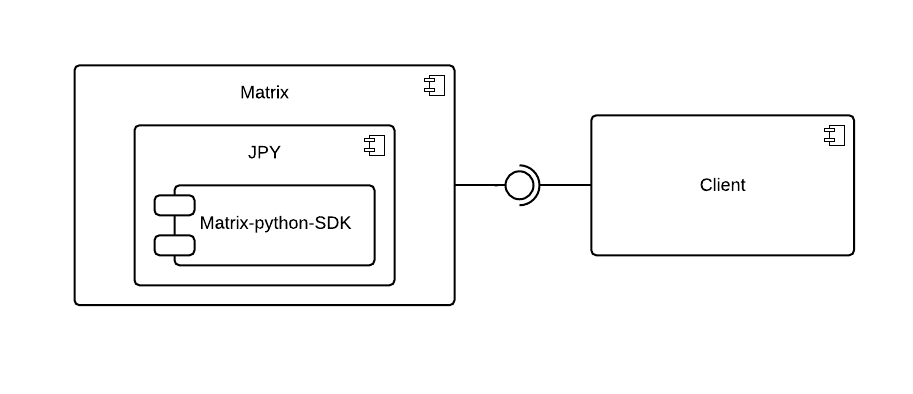
\includegraphics[width=14cm]{figures/matrix_component.png}
	\caption{Component diagram for the system}
	\label{fig:matrix_component}
\end{figure}

Matrix provides several SDK libraries that client application can be build on top of. The most prominent is the Javascript Matrix SDK. It is the best maintained with the largest feature set however it is not compatible with the Java based Information-Flow Control tool Paragon. A Java Matrix SDK exists but it is an early alpha version with end-to-end encryption not implemented yet. The Python Matrix SDK is another major SDK with support for end-to-end encryption in beta. The Python Matrix SDK is used in the Matrix component through a Java-Python bridge \emph{JPY} that can embed Python code in Java as shown in the Matrix component in figure \ref{fig:matrix_component} 


\subsubsection{Matrix}
%Matrix API's
% A lot of things are handled under the hood by the matrix SDK.
Matrix is an important component in the system. It manages the transmission and storage of patient journals through rooms while managing end-to-end encryption. The encryption mechanism is automatically provided and the SDK manages the session keys under the hood.  As described in section \ref{matrix:architecture} a room is a conceptual place for sending an receiving events and events can be any of any structure. The event history in a rooms is replicated at each homeserver. 

The following design choices and assumptions are made regarding Matrix and the system: 

\begin{itemize}
	\item A homeserver represents a hospital server that replicates the history of a patient journal. 
	\item A room represents a single patient journal's version history.
	\item An event represents a patient journal.  
	\item The latest event in a room is the global state of the patient journal.
	\item A hospital is represented by a single matrix user that participates in a room.
	\item A hospital's matrix user is used by doctors and secretaries to access patient journals. 
\end{itemize}


The room can be considerably large since many different types of hospitals needs access to a patient journal. This puts a lot of responsibility on securing the endpoints but also adds concern to who controls the rooms and how hospitals are added. It is assumed that a central authority would be managing all room whom all participants in the room trust. That authority would be the government which are responsible for creating and managing the rooms. Only the authority can invite and remove Hospitals from a room. Hospitals can only join a room if they have been invited.


\subsubsection{Client}

%Program flow
%Program starts as either a Doctor or secretary. If Doctor then IsDoctor is opened.
%The program runs a while loop and presents a list of patients which the user can select.
%When user selects a journal it is first checked who the user is.
%If the user is doctor then it is checked if the patient is referred and the lock IsReferred would then open
%The user then receives the journal through the receive method and can perform some action: 
%If the user is a secretary than the user can print the journal, or edit the public note.
%If the user is a doctor then the journal can be printed, public note can be edited or 
%a public session note can be added. If the patient is referred then the doctor can add to private session
%When the user has done some action the program returns to the main loop.  


 The hospital keeps track of all journals they have access to through a hashmap with key being the CPR and the value being the roomid. When a doctor or secretary want to retrieve a journal; the latest journal from the patient journal's room is fetched.
 he hospital retrieves the latest event 
 
 
 
The sessions between a doctor and a 

A patient journal the PatientJournal class depicts 

% Describe how the design with matrix would be
Figure \ref{fig:journalsystem} depicts the class diagram for the system.



\begin{figure}[H] 
	\hspace*{-1.3cm}
	\centering
	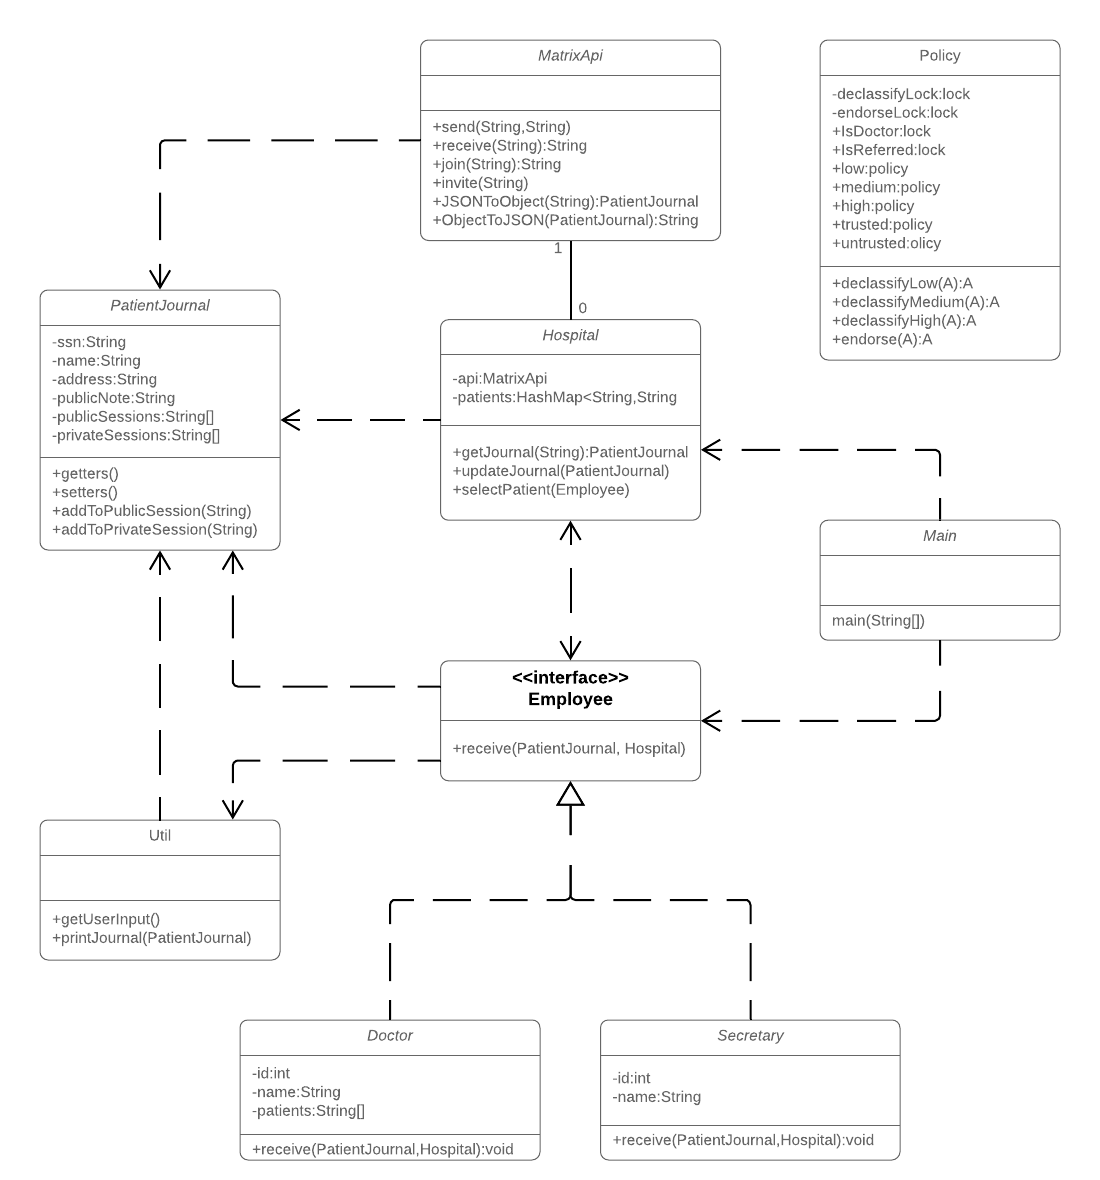
\includegraphics[width=14cm]{figures/journalsystem_class.png}
	\caption{Class diagram for the Journal system}
	\label{fig:journalsystem}
\end{figure}





\subsubsection{Limitations}

%Incompatibility with Paragon


A design problem is the concurrent writes to a journal from multiple hospital. Before writing to a journal; the latest version of the journal in Matrix is first retrieved and then the writes are appended to the journal. However multiple hospitals might have retrieved the latest journal and different doctors might have committed changes to the journal and send it to Matrix hence one of the writes would be lost since only the latest journal is retrieved. 

%Another limitation is that the rooms a hospital can access are precreated and the hospitals in a room are preconfigured. 

%This is a common issue in distributed systems but is not handled in this solution. 


% It is assumed that a version control mechanism is in place and the latest journal received is always up to date.
% Solution merging data like version control systems like git.


\newpage
\section{Paragon implementation}

A \emph{policy-first} approach is used when implementing the prototype. The first step is to carefully specify the policies for the system. A journal has several parts that may only be obtained by appropriate users; the policies should uphold that. The policies are defined in the class \emph{Policy} and used throughout the system.

For confidentiality three policies are defined with \emph{low} being the most liberal, \emph{High} being the most strict and \emph{medium} in the middle. The figure \ref{fig:lattice_confidentiality} depicts a lattice for the three policies where information can only flow upwards. In the figure \emph{public} represents low, \emph{confidential} represents medium and \emph{secret} represents high. 

Based on the requirements the information labeled with secret should only be obtainable by the Doctor that the patient has been referred to. There could be defined a similar independent secret labels e.g. for information that only the patient's psychiatrist could view.  

% Show confidentiality lattice and combined lattice.

\begin{figure}[H] 
	\centering
	\includegraphics[width=6cm]{figures/lattice_confidentiality.png}
	\caption{Lattice in the system}
	\label{fig:lattice_confidentiality}
\end{figure}

The lattice in figure \ref{fig:lattice_confidentiality}b illustrates the integrity policy and states that data labeled as \emph{untrusted} can not flow to \emph{trusted}. The trusted and untrusted labels serves the purpose of disallowing flows to the journal.

The fields in the PatientJournal class are decorated with a combination of confidentiality labels. The \emph{product lattice} is illustrated in the figure \ref{fig:lattice_product}.

\begin{figure}[H] 
	\centering
	\includegraphics[width=7cm]{figures/lattice_product.png}
	\caption{Product lattice}
	\label{fig:lattice_product}
\end{figure}


The next section will show how the policies have been defined and used in paragon. 



\subsection{Policies}\label{policies} 

In Paragon a policy defines what actor information can flow to and under what conditions 
\cite{paragonprogramming}. Any object can be used as an actor. The confidentiality policies in the prototype uses \emph{Doctor} and \emph{Secretary} as actors. 


\subsubsection{Defining policies}\label{policydef}
The policies \emph{low}, \emph{medium} and \emph{high} are defined as this:

\begin{lstlisting}
public static final policy low = { Doctor d: ;Secretary s:};
public static final policy medium = { Doctor d:};
public static final policy high = { Doctor d: IsReferred(d)};
\end{lstlisting}


Here policy \emph{low} is less restrictive than \emph{medium} since a variable labeled with the policy low can be viewed by the any\emph{Doctor} or \emph{Secretary} actor whereas a variable labeled with \emph{medium} can only be viewed by any \emph{Doctor} actor. The policy \emph{high} is a more interesting policy. It is more restrictive since it can only flow to a specific \emph{Doctor} if the lock \emph{IsReferred(d)} is open. Policy \emph{high} is an example of a dynamic policy which uses a parameterized unary lock.

The following are integrity policies defined as follows:
\begin{lstlisting}
private static final Object untrustedObserver = new Object();
private static final Object trustedObserver = new Object();
public static final policy untrusted = { untrustedObserver :; };
public static final policy trusted = { untrustedObserver :; trustedObserver: };
\end{lstlisting}


The actors used here are \emph{untrustedObserver} and \emph{trustedObserver}. The policy \emph{trusted} can be viewed by both observers while \emph{untrusted} can only be viewed by \emph{untrustedObserver}. This captures integrity since a variable labeled with \emph{untrusted} can not flow to \emph{trusted}. Note that actors used here are instances of objects and using them as actors gives the policies a special property of being combinable with other policies \cite{paragonprogramming}.


% The policies defined for confidentiality are with fresh actors and the objects correspond to the entities where information may flow. By using fresh actors the policies can be combined with other policies that would otherwise have interfered with eachother. The integrity policy is more general in nature and has defines two actors; trusted and untrusted observers. The policies are defined as follows: ?(Policy.high + Policy.trusted).

% Dynamic policy is used for when a doctor adds notes to session. The lock IsDoctor must be open for the method addToSession() can be invoked. This is checked at runtime as seen in the code snippet:


% Policy definition
% Policy usage
\subsubsection{Using policies}
A policy is used as a label on variables. To express concerns for both confidentiality and integrity the policies described previously can be combined and labeled on variables. Fields in the class \emph{PatientJournal} are defined as:

\begin{lstlisting}
	private ?(Policy.low    + Policy.trusted) String   publicNote;
	private ?(Policy.medium + Policy.trusted) String[] publicSessions;
	private ?(Policy.high   + Policy.trusted) String[] privateSessions;
\end{lstlisting}

The \emph{PatientJournal} class has methods that adds a session to \emph{publicSession} or \emph{privateSession}. The class also implements simple getter and setter methods. Common for these methods are they must specify the \emph{read} or \emph{write} effect for the method.

% Show table of policies and how they are defined and how they are used for low, high and medium.



\subparagraph{Read effects}
The read effect specifies what the information policy is. It has already been introduced when labeling the fields in the \emph{PatientJournal} class. When decorating a method with a read effect signature it simply tells what the policy is for the returned type. Paragon ensures that the policy returned must respect the policies of the field or parameters that are in the context of the method. Through read effects explicit flows are captured across methods and fields. This is an example of how a simple \emph{get()} method is defined in \emph{PatientJournal}.
\begin{lstlisting}
?(Policy.medium + Policy.trusted)
public  String[] getPublicSessions(){
	return publicSessions;
}
\end{lstlisting}

If the read effect instead was \emph{?(Policy.low+Policy.trusted)} then Paragon would have caught it since the field \emph{publicSession} has a more restrictive policy. Note that is a read effect is not specified then Paragon sets the read effect as \emph{?(Object x:)} (the least restrictive policy in Paragon).

\subparagraph{Write effects}
In Paragon the write effect prevents implicit flows. The write effect specifies what context the method can be called in. The context would have to at least as restrictive as the method write effect. The write effect for a method is defined like this:

\begin{lstlisting}
!(Policy.lowD + Policy.trusted) 
public void setPublicNote(?(Policy.lowD + Policy.trusted) String note){
	this.publicNote = note;
}
\end{lstlisting}

This method has the write effect \emph{!(Policy.lowD+Policy.trusted)}. Now if this method was called in a method that has the write effect \emph{!(Policy.highD+Policy.trusted)} then there would be an implicit flow and Paragon would detect it.

Read and write effects are important aspect of Paragon since they ensure secure information flow across methods and fields.

\subsection{Locks}
%Integrity. Are used for ensuring that data from untrusted sources can not interfere with trusted. Only used for input. Integrity of who can declassify what information is based dynamically enforced through locks.
%How locks are openend
% Show table for locks and how they are defined and how they are used.
% IsReferred is used to check if the current doctor has the patient in care
% It opens the lock Referred.
% Would be a problem in a concurrent system then the Referred lock would be shared by multiple users at the same time. Another design would be to have a list of global users or what? 

% Primary mechanism for ensuring integrity and the trusted untrusted labeling for mainly input.


\subsection{Declassification}

\begin{table}[H]
	\hspace*{-2cm}
	\centering
	\begin{tabular}{|l|l|l|l|l|} 
		\hline
		& Who               & What                                                                                                   & Where                                                                         & When                       \\ 
		\hline
		1 & Anyone~           & \begin{tabular}[c]{@{}l@{}}Journal.Name\\Journal.SSN\\Journal.Address\\Journal.PublicNote\end{tabular} & Util.printJournal()                                                           & Printing the journal       \\
		& Doctor            & Journal.PublicSessions                                                                                 & Util.printJournal()                                                           & Printing the journal       \\
		& Doctor (Referred) & Journal.PrivateSessions                                                                                & Util.printJournal()                                                           & Printing the journal       \\
		&                   &                                                                                                        &                                                                               &                            \\ 
		\hline
		2 & Anyone            & User input                                                                                             & \begin{tabular}[c]{@{}l@{}}secretary.receive()\\doctor.receive()\end{tabular} & After prompting for input  \\
		&                   &                                                                                                        &                                                                               &                            \\
		\hline
	\end{tabular}
\end{table}

% Declassification is necessary for the input and output channels. The journals might be print to the user over the output channel. In order to do so the journal must be declassified correctly. 

%Another concern is the input channel where the input needs to be endorsed. The client requires input from both secretary and doctor. Input channels are untrusted and need to be endorced/sanitized based on which actor the input came from.

% The following table shows the rules for declassification and endorsement throughout the system.




%\subsubsection{Lattice}

\subsection{Limitations}

\subsubsection{Matrix API}


\subsubsection{Exception handling}
Exception handling



%\subsection{Exception handling}
 
 
%Technical requirements: -Msg type should be "m.text" when sending patient journal (JSON format). The convertion of string to JSON and vice versa should happen in the client.

\section{Summary}